% main file
\documentclass[12pt, twoside, a4paper, openright]{book}
\usepackage[utf8]{inputenc} % Compatibility for spanish accents

%%%%%%%%%%%%%%%%%%%%%%%%%%%
%%% Start Configuration %%%
%%%%%%%%%%%%%%%%%%%%%%%%%%%

\newcommand{\egilea}{Haritz Medina}
\newcommand{\izenburua}{Sheetchat - Generación de chatbots a partir de hojas de cálculo.}
\newcommand{\masterDate}{2016}
\newcommand{\masterName}{Sistemas Informáticos Avanzados}
\newcommand{\masterSpecialization}{Sistemas distribuidos y web}

% Comment unused languages
%\newcommand{\documentLanguageBasque}{eu}
\newcommand{\documentLanguageSpanish}{es}
%\newcommand{\documentLanguageEnglish}{en}

% Codificación del archivo / fitxategiaren kudeaketa
\usepackage{ucs}
\usepackage[T1]{fontenc}


% ################################################################
% #######     SIZE OF THE PAGES                     ##############
% ################################################################
\usepackage[left=3.5cm, right=2.5cm, top=4.0cm, bottom=3.0cm]{geometry}
% \usepackage[left=1.5cm, right=2.5cm, top=2.0cm, bottom=2.0cm]{geometry}


% ################################################################
% #######     HEADERS                               ##############
% ################################################################
\usepackage{fancyhdr}           % Para cambiar las cabeceras de las pginas

\pagestyle{fancy}
\renewcommand{\chaptermark}[1]{ \markboth{#1}{} }
\renewcommand{\sectionmark}[1]{ \markright{#1}{} }

\fancyhf{}
\fancyhead[LE,RO]{\thepage}
\fancyhead[RE]{\textit{ \nouppercase{\leftmark}} }
\fancyhead[LO]{\textit{ \nouppercase{\rightmark}} }

\fancypagestyle{plain}{ %
  \fancyhf{} % remove everything
  \renewcommand{\headrulewidth}{0pt} % remove lines as well
  \renewcommand{\footrulewidth}{0pt}
}


	% Redefine plain page style
	\fancypagestyle{plain}{
		\fancyhf{}
		\renewcommand{\headrulewidth}{0pt}
		\fancyfoot[LE,RO]{\thepage}
	}

	% Define pagestyle
	\pagestyle{fancy}
	\fancyhf{}
	% \renewcommand{\chaptermark}[1]{\markboth{ \emph{#1}}{}}
	\fancyhead[LO]{}
	\fancyhead[RE]{\leftmark}
	\fancyfoot[LE,RO]{\thepage}

	% Code for creating empty pages
	% No headers on empty pages before new chapter
	% \makeatletter
	% \def\cleardoublepage{\clearpage\if@twoside \ifodd\c@page\else
		% \hbox{}
		% \thispagestyle{plain}
		% \newpage
		% \if@twocolumn\hbox{}\newpage\fi\fi\fi}
	% \makeatother \clearpage{\pagestyle{plain}\cleardoublepage}

	% Otra opción: considerar si funciona
	% this next section (till \makeatother) makes sure that blank pages
	%% are actually completely blank, cause they're not usually
	\makeatletter
	\def\cleardoublepage{\clearpage\if@twoside \ifodd\c@page\else
		\hbox{}
		\vspace*{\fill}
		\thispagestyle{empty}
		\newpage
		\if@twocolumn\hbox{}\newpage\fi\fi\fi}
	\makeatother


	% \pagestyle{fancy}				% use fancyhdr style
	% \setlength{\headheight}{13pt}

	% Limpiar estilo actual
	% \fancyhead{}
	% \fancyfoot{}
	% % or \fancyhf{}

	% \renewcommand{\headrulewidth}{0.4pt}    % Cabecera: subraya la cabecera (fijar en "0pt" si no se desea).
	% \renewcommand{\footrulewidth}{0pt}      % Pié: subraya el pie de página (fijar en "0pt" si no se desea).

	% There are seven letters you need to know before you can define your own header/footer:
	% E: Even page
	% O: Odd page
	% L: Left field
	% C: Center field
	% R: Right field
	% H: Header
	% F: Footer

% 	\fancyhead[CO,CE]{---Draft---}
% 	\fancyfoot[CO,CE]{Confidential}

% 	\fancyfoot[RO, LE] {\thepage}
% 	% or \fancyhf[FRO,FLE]...
% 
% 	\fancyhead[RE]{\nouppercase{\leftmark}}	% Cabecera: incluye información del nivel superior (Capítulo) % a la derecha (R) de las páginas pares (E), evitando escribir % todo en mayúsculas (que sería la opción por defecto).
% 	% or \fancyhf[HRE]...
% 
% 	\fancyhead[LO]{\nouppercase{\rightmark}}% Cabecera: incluyer información del nivel inferior (Sección) % a la izquierda (L) de las páginas impares (O), evitando escribir % todo en mayúsculas (que sería la opción por defecto).

	% \renewcommand{\chaptermark}[1]{%
		% \markboth{\small\slshape\chaptername{} \thechapter: #1}{}
		% }
	% \renewcommand{\sectionmark}[1]{%
		% \markright{\small\slshape\thesection : #1}
		% }

\renewcommand{\chaptermark}[1]{\markboth{#1}{}}
\renewcommand{\sectionmark}[1]{\markright{\thesection\ #1}}


%% which sections are numbered
\setcounter{secnumdepth}{2}

 
% ################################################################
% #######     Bibliografia                          ##############
% ################################################################
% \usepackage{natbib}
% \newcommand{\citenp}[2][ ]{\citeauthor{#2}#1 (\citeyear{#2})}
% \bibpunct{}{}{;}{a}{,}{,~}
% \newcommand{\myetal}{\emph{et~al.}}
% \bibliographystyle{plainnat4}
\bibliographystyle{apalike}


% To insert development comments (todos, corrections...)
\usepackage[textsize=scriptsize,textwidth=2cm]{todonotes}
% How to use: 
% - \todo{comentario/iruzkina} (insert into tex)
% - \todo[inline]{}

% ################################################################
% #######     FONT TYPES                            ##############
% ################################################################
% Charter
%\usepackage[bitstream-charter]{mathdesign}
% 	\renewcommand{\rmdefault}{mdbch} % charter
\DeclareSymbolFont{usualmathcal}{OMS}{cmsy}{m}{n}
\DeclareSymbolFontAlphabet{\mathcal}{usualmathcal}
%\usepackage{charter}
% \renewcommand{\rmdefault}{bch}
% \renewcommand{\bfdefault}{b}

% times erabili beharrean
\usepackage{mathptmx}
\usepackage[scaled=.90]{helvet}

% \renewcommand{\rmdefault}{ppl}
% \usepackage{mathpazo} % palatino
% \linespread{1.05}        % Palatino needs more leading
% \usepackage[bitstream-charter]{mathdesign}
% \usepackage{libertine}

%\usepackage[scaled]{berasans}

%\usepackage[scaled]{beramono}
% \renewcommand{\sfdefault}{fxbf}
	% libertine
% 		\renewcommand{\rmdefault}{fxlj} % Linux libertine 


% Sans serif


% ################################################################
% #######     GRAPHICS                              ##############
% ################################################################
\usepackage{graphicx}
\DeclareGraphicsExtensions{.png,.gif,.jpg,.pdf}
% \graphicspath{./irudiak/}
% \newcommand{\irudia}[3]{%
	% \begin{figure}[htb!]
	% \centering%
	% \includegraphics[width=#2]{#1}
	% \caption{#3}
	% \label{fig:#1}
	% \end{figure}
% }

\usepackage[figuresright]{rotating}

\newcommand{\fitx}[1]{\texttt{#1}}

%%%%%%%%%%%%%%%%%%%%%%%%%%%%%%%%%%%%%%%%%%%%%%%%%%%%%%%%%%%%%%%%
%%%%%%%%%%%  PARRAFOEN ESTILOA    %%%%%%%%%%%%%%%%%%%%%%%%%%%%
\frenchspacing
\widowpenalty=1000

% \titlespacing{\section}{1pc}{0ex plus .1ex minus .2ex}{1pc}
% \titlespacing{\section}{0pt}{*1}{*1}
\setlength{\parindent}{0cm} % anula indentacion de parrafos
\setlength{\parskip}{1.5ex plus 0.5ex minus 0.5ex}   % establece separacion entre parrafos a 8 puntos

\setlength\headheight{15pt}

\usepackage{setspace} % Lerroen arteko espazioa
%\singlespacing
\onehalfspacing
%\doublespacing
%\setstretch{1.1}

% hobeto ``justifika''tzeko
%\usepackage[protrusion=true,expansion=true]{microtype}


%%%%%%%%%%%%%%%%%%%%%%%%%%%%%%%%%%%%%%%%%%%%%%%%%%%%%%%%%%%%%%%%
%%%%%%%%%%% IZENBURUEN ESTILOA   %%%%%%%%%%%%%%%%%%%%%%%%%%%%
\usepackage[sf,outermarks]{titlesec}
% \usepackage[compact]{titlesec}

\titleformat{\chapter}[display]
  {\bfseries\Large}
  {\filleft\Huge\thechapter. \Large\MakeUppercase{\chaptertitlename}}
  {4ex}
  {\titlerule
	\vspace{2ex}%
	\filright}
  [\vspace{2ex}%
   \titlerule]

% ATalen formatua
\renewcommand{\thepart}{\arabic{part}}
\titleformat{\part}[display]
  {\bfseries \Large}
  {\filcenter \Huge\thepart. \Huge\MakeUppercase{\partname}}
  {4ex}
  {%marra
    \vspace{2ex}%
    \filcenter \huge  \filright} %filcenter
  [\vspace{2ex}%
   ]





%usepackage{calc} % para hacer calculos al establecer las medias ej: \textwidth -2px
% \usepackage{sectsty}
% \newcommand{\cabecerasformatosection}[1]{%
	% {\makebox[0.98\linewidth][l]{#1}}
% }
% \newcommand{\cabecerasformatosubsection}[1]{%
	% {\makebox[0.98\linewidth][l]{\textsl{#1}}}
% }
% \newcommand{\cabecerasformatosubsubsection}[1]{%
	% {\framebox[1.1\width][l]{#1}}
% }
% \sectionfont{\cabecerasformatosection}
% \subsectionfont{\cabecerasformatosubsection}
% \subsubsectionfont{\cabecerasformatosubsubsection}
% \sectionfont{\sffamily}
% \subsectionfont{\sffamily\textsl}
% \subsubsectionfont{\sffamily}


\usepackage{appendix}
% \usepackage{glossaries}
% Erabilera 
% http://en.wikibooks.org/wiki/LaTeX/Glossary
% latexmk erabiliz gero, ikusi http://tex.stackexchange.com/questions/1226/how-to-make-latexmk-use-makeglossaries

% Glosario-en eskuliburu zabaldua
% http://osl.ugr.es/CTAN/macros/latex/contrib/glossaries/glossaries-user.html#x1-140002.2



\usepackage{color}  
\usepackage{xcolor}
\usepackage{colortbl}

\definecolor{light-gray}{cmyk}{0,0,0,.3} 
\definecolor{orange}{rgb}{1,0.7,0}
\definecolor{light-brown}{RGB}{184,134,11}

\definecolor{gray90}{gray}{.90}
\definecolor{gray75}{gray}{.75}
\definecolor{gray95}{gray}{.95}

\definecolor{lightgray}{gray}{.8}
\definecolor{lightlightgray}{gray}{.95}

\definecolor{atzekokolorea}{gray}{.97}
\definecolor{atzekokoloreasol}{gray}{.7}
\definecolor{atzekokoloreafitx}{gray}{.97}
\definecolor{atzekokoloreafitx_markoa}{gray}{.65}

\usepackage{textcomp} % XML kodea formateatzeko

\usepackage{listings}

\lstset{
    tabsize=4,
    basicstyle=\scriptsize,
    upquote=true,
    aboveskip={1.5\baselineskip},
    columns=fixed,
    showstringspaces=false,
    extendedchars=true,
    breaklines=true,
    showtabs=false,
    showspaces=false,
    showstringspaces=false,
    identifierstyle=\ttfamily,
    commentstyle=\color[rgb]{0.133,0.545,0.133},
    stringstyle=\color[rgb]{0.627,0.126,0.941}\ttfamily,
    morekeywords={SCORE},keywordstyle=\color{red},
    emph={SCORE,CODE,ID,LEMA,POS},emphstyle=\color{light-brown},
    moreemph={[2]top,num,ENtitle,TERM,WF,SYNSET,ENdesc,ENnarr,EStitle,ESdesc,ESnarr,EXP,DOC,DOCNO,DOCID,HEADLINE,TEXT},emphstyle={[2]\color{blue}}
}



\lstset{ frame=Ltb,
     framerule=0pt,
     aboveskip=0.5cm,
     framextopmargin=3pt,
     framexbottommargin=3pt,
     framexleftmargin=0.4cm,
     framesep=0pt,
     rulesep=.4pt,
     backgroundcolor=\color{gray90},
     rulesepcolor=\color{black},
     %
     stringstyle=\ttfamily,
     showstringspaces = false,
     basicstyle=\small\ttfamily,
     commentstyle=\color{gray45},
     keywordstyle=\bfseries,
     %
     numbers=left,
     numbersep=15pt,
     numberstyle=\tiny,
     numberfirstline = false,
     breaklines=true,
   }
 
\lstnewenvironment{listing}[1][]
   {\lstset{#1}\pagebreak[0]}{\pagebreak[0]}
\lstdefinestyle{consola}
    {
        numbers=none,
        xleftmargin=\parindent,
        xrightmargin=\parindent,
        aboveskip=3mm,
        belowskip=0.01mm,
        basicstyle=\scriptsize\bf\ttfamily,
        backgroundcolor=\color{gray75}
    }
\lstdefinestyle{no_fileconf}
{
    numbers=none,
    xleftmargin=\parindent,
    xrightmargin=\parindent,
    aboveskip=3mm,
    belowskip=0.01mm,
    basicstyle=\footnotesize\ttfamily,
    backgroundcolor=\color{gray90},
}
\lstdefinestyle{fileconf}
{
        xleftmargin=\parindent,
        xrightmargin=\parindent,
        aboveskip=3mm,
        belowskip=0.01mm,
        basicstyle=\footnotesize\ttfamily,
        backgroundcolor=\color{gray95},
}

\lstset{
	float=[*],
	lineskip=0pt,
	inputencoding=utf8x,
	extendedchars=\true,
% 	texcl=true,
    basicstyle=\scriptsize\ttfamily,             % print whole listing small
	backgroundcolor=\color{atzekokolorea},
	framesep=3pt,frame=single,framerule=0.6pt,framexleftmargin=1pt,
	tabsize=4, 
	linewidth=0.98\linewidth,
	xleftmargin=5pt,
	breaklines=true,
	moredelim=[il][\sffamily\scriptsize\slshape\itshape\color{GRISARGIA}]{º},
	moredelim=[is][\bfseries]{ª}{ª},
%     keywordstyle=\color{black}\bfseries,
% 	fontadjust=true,
                                   % underlined bold black keywords
%     identifierstyle=,              % nothing happens
%     commentstyle=\color{white}, 	% white comments
%     stringstyle=\ttfamily,         % typewriter type for strings
%     showstringspaces=false,        % no special string spaces
%     showtabtruee,        % no special string spaces
% 	upquote=true,
	keepspaces=true,
	% showspaces=true,
	% showtabs=true,
	columns=fullflexible
	}

\lstset{
  literate={á}{{\'a}}1
           {é}{{\'e}}1
           {í}{{\'i}}1
           {ó}{{\'o}}1
           {ú}{{\'u}}1
		   {ñ}{{\~{n}}}1
}


% \renewcommand*\thelstnumber{(\the\value{lstnumber})}

% \lstnewenvironment{komandoak}{\lstset{upquote=true,escapechar=}}{}
% ,numbers=left, stepnumber=1, numbersep=5pt
\lstnewenvironment{komandoak}{
	\lstset{
			upquote=true,
			escapeinside={(!}{!)},
% 			escapebegin=\begin{bfseries},escapeend=\end{bfseries},
% 			morecomment=[l]{\#},
% 			commentstyle=\itshape,
			frameround=tttt
				}}{}


\usepackage{longtable}
\usepackage{multirow}
\usepackage{multicol}

\usepackage{tabulary}

\usepackage{amsmath}
\usepackage{url}
\usepackage{bm} % bold maths symbols

\usepackage{paralist} % compactenum...
\usepackage{booktabs} %\tauletan \toprule, \bottomrule...
% \usepackage{algorithmic} % algoritmoen zerrenda lortzeko
% \usepackage{algorithm} % algoritmoen zerrenda lortzeko

% \usepackage{soul} % text highlighting \hl

% \usepackage[Bjornstrup]{fncychap} 
% \ChTitleVar{\raggedleft\LARGE\bfseries}

\usepackage{tocbibind} % hau ez badut jartzen, gaien aurkibidea eta bibliografia ez dira agertzen pdf-ko bookmark-ean

% ################################################################
% #######     HIZKUNTZA / IDIOMA                    ##############
% ################################################################


% Cover translatable text
\ifdefined\documentLanguageBasque
	\providecommand{\upvehu}{Euskal Herriko Unibertsitatea UPV/EHU}
	\providecommand{\gradua}{\masterName}
	\providecommand{\mapizenburua}{Master Amaierako Tesia}
	\providecommand{\informatikafakultatea}{Informatika Fakultatea}
	\providecommand{\abstract}{Laburpena}
	\providecommand{\authorLabel}{Egilea}
	\providecommand{\directorLabel}{Zuzendaria}
\fi
\ifdefined\documentLanguageSpanish
	\providecommand{\upvehu}{Universidad del País Vasco UPV/EHU}
	\providecommand{\mapizenburua}{Tesis fin de Máster}
	\providecommand{\informatikafakultatea}{Facultad de Informática}
	\providecommand{\abstract}{Resumen}
	\providecommand{\authorLabel}{Autor}
	\providecommand{\directorLabel}{Director}
\fi
\ifdefined\documentLanguageEnglish
	\providecommand{\upvehu}{University of the Basque Country UPV/EHU}
	\providecommand{\mapizenburua}{Master's degree Thesis}
	\providecommand{\informatikafakultatea}{Faculty of Computer Science}
	\providecommand{\abstract}{Abstract}
	\providecommand{\authorLabel}{Author}
	\providecommand{\directorLabel}{Supervisor}
\fi

\usepackage[font=small,labelfont=bf]{caption}

% General translatable text and properties
\ifdefined\documentLanguageBasque
	\usepackage[basque]{babel}
	\addto\captionsbasque{
		\renewcommand{\contentsname}{Gaien aurkibidea}
		\renewcommand{\listfigurename}{Irudien aurkibidea}
		\renewcommand{\listtablename}{Taulen aurkibidea}
		%\renewcommand{\listalgorithmname}{Algoritmoen zerrenda}
		\renewcommand{\appendixname}{Eranskina}%
		\renewcommand{\appendixpagename}{Eranskinak}
		\renewcommand{\appendixtocname}{Eranskinak}
		\renewcommand{\bibname}{Bibliografia}
		\renewcommand{\abstractname}{Laburpena}
		%% Hau ez badut jartzen, Irudia eta Taula maiuskulaz jartzen ditu
		\renewcommand{\tablename}{Taula}
		\renewcommand{\figurename}{Irudia}
		% Glosategietarako
		% \renewcommand*{\glossaryname}{Glosategia}%
		% \renewcommand*{\acronymname}{Akronimoa}%
		% \renewcommand*{\entryname}{Notazioa}%
		% \renewcommand*{\descriptionname}{Deskribapena}%
		% \renewcommand*{\symbolname}{Symboloa}%
		% \renewcommand*{\pagelistname}{Orri zerrenda}%
		% \renewcommand*{\glssymbolsgroupname}{Symboloak}%
		% \renewcommand*{\glsnumbersgroupname}{Zenbakiak}%
		% Sections
		\providecommand{\introduction}{Sarrera}
		\providecommand{\conclusions}{Ondorioak}
	}
	%% Captionak euskarazko ordenean
	\DeclareCaptionLabelFormat{euskaraz}{#2\bothIfSecond{\nobreakspace}{#1}}
	\captionsetup{labelformat=euskaraz}
\fi

\ifdefined\documentLanguageSpanish
	\usepackage[spanish]{babel}
	\addto\captionsspanish{
		\renewcommand{\contentsname}{Índice de capítulos}
		\renewcommand{\listfigurename}{Índice de figuras}
		\renewcommand{\listtablename}{Indice de tablas}
		%\renewcommand{\listalgorithmname}{Índice de algoritmos}
		\renewcommand{\appendixname}{Anexo}
		\renewcommand{\appendixpagename}{Anexos}
		\renewcommand{\appendixtocname}{Anexos}
		\renewcommand{\bibname}{Bibliografía}
		\renewcommand{\abstractname}{Resumen}
		% Sections
		\providecommand{\introduction}{Introducción}
		\providecommand{\conclusions}{Conclusiones}
	}
	
	% tabla de contenido sin numeracion 
	% \renewcommand\contentsname{Tabla de contenido}
	% lista de figuras 
	% \renewcommand\listfigurename{Lista de figuras}
	% \clearpage

	% lista de tablas
	% \renewcommand\listtablename{Lista de tablas}
		% \renewcommand{tablename}{tabla}
\fi

\ifdefined\documentLanguageEnglish
	\usepackage[english]{babel}
	% Sections
	\providecommand{\introduction}{Introduction}
	\providecommand{\conclusions}{Conclusions}
\fi

\usepackage[hyperindex,bookmarks,colorlinks=true,citecolor=blue,urlcolor=blue,linkcolor=blue,pdftex,unicode]{hyperref}

\hypersetup{
	pdfauthor = {\egilea},
	pdftitle = {\izenburua},
	pdfsubject = {\mapizenburua - \informatikafakultatea},
	pdfkeywords = {\today},
	pdfcreator = {},
	pdfproducer = {}
}

% \makeglossaries	% according to manual, in the preamble and after hyperref

% line in order to check if utf-8 is properly configured: áéíóúñ


%%%%%%%%%%%%%%%%%%%%%%%%%
%%% End configuration %%%
%%%%%%%%%%%%%%%%%%%%%%%%%

\title{\izenburua}
\author{\egilea}


\begin{document}
\frontmatter
% \maketitle
\thispagestyle{empty}

\newcommand{\HRule}{\rule{\linewidth}{0.5mm}} 

% Aurrekariak
\begin{center}
  \includegraphics[width=0.5\textwidth]{template/figs/ehu-logo-osoa.jpg} \\[1.3cm]
  % \textsf{\upvehu}\\[0.15cm]
   {\Large \masterName}\\
   {\masterSpecialization}\\[1.5cm]

  {\large {\mapizenburua}}\\[0.2cm]
\HRule \\[0.5cm]

% Titulua
{ \LARGE 
\begin{spacing}{1}
  \textbf{\izenburua}
\end{spacing}
}
 \vspace{0.5cm}
\HRule \\[1.0cm]

% Egilea
{ \authorLabel\\}
{\Large \textsl{\egilea}}
\vspace{2.0 cm}

\includegraphics[width=0.35\textwidth]{template/figs/logo_infor.pdf} \\[0.1cm]
%Urtea
% \vfill
{\large \textsf{\masterDate}}

\end{center}

% line in order to check if utf-8 is properly configured: áéíóúñ

\cleardoublepage


\chapter*{\abstract}
\addcontentsline{toc}{chapter}{\abstract}
\setcounter{page}{1}
% \thispagestyle{empty}

Las hojas de cálculo son herramientas que tienen un uso extendido con más de 750 millones de usuarios a lo largo del mundo. Permiten crear complejas simulaciones, modelar situaciones financieras o analizar y mostrar datos a clientes. Sin embargo son herramientas que dentro del mundo móvil son muy demandadas pero complejas de utilizar. Recientes estudios afirman que cerca de un 80\% de los usuarios de hojas de cálculo no disponen de un ordenador cuando necesitan consultar datos almacenados en hojas de cálculo. En este trabajo se ha definido un DSL y una aplicación llamada SheetChat que permite a un usuario definir y generar sus propios chatbots que le ayuden a consultar datos de su hoja de datos en una configuración móvil. Se han desarrollado tres casos de uso en tres contextos diferentes donde se evalúa la herramienta.


\textbf{Palabras clave:} SpreadSheets, Chatbot, Mobile Setting

% line in order to check if utf-8 is properly configured: áéíóúñ

\cleardoublepage

% Remove parskip for toc
% \setlength{\parskip}{0ex plus 0.5ex minus 0.2ex}
\setcounter{tocdepth}{2}	% Titles level degree at table of contents
\tableofcontents			% Show a table of contents

\newpage
\listoffigures

\newpage
\listoftables

% Change to a more spaced text-style
\setlength{\parskip}{1.3ex plus 0.2ex minus 0.2ex}
\renewcommand{\baselinestretch}{1.3}

	\fancyhf{}
	\fancyhf[OLH]{\rightmark}
	\fancyhf[ERH]{\leftmark}
	\fancyhf[ORH,ELH]{\thepage}

\mainmatter

%%%%%%%%%%%%%%%%%%%%%
%%% Content files %%%
%%%%%%%%%%%%%%%%%%%%%
\chapter{\introduction}

% TODO Revision and fix

La inclusión del Smartphone como herramienta de comunicación y búsqueda de información se ha extendido superando a los sistemas de cómputo tradicionales como el PC o los portátiles. El Smartphone dispone actualmente una capacidad de trabajo similar a los PC con la ventaja de la movilidad que ofrece. En la actualidad, con un Smartphone se pueden realizar la mayoría de tareas cotidianas que un usuario puede requerir, como leer el correo electrónico, comunicarse con sus seres queridos, consultar información en la web o realizar compras online.

Sin embargo, a pesar de que se puedan realizar tareas complejas, sus limitaciones provoca que algunas tareas puedan ser realmente tediosas o imposibles de realizar. Un ejemplo claro es la consulta de información de datos en hojas de cálculo. En la actualidad el uso de hojas de cálculo como Microsoft Excel o Google Spreadsheet es una de las herramientas más utilizadas en el manejo de información, en el ámbito empresarial, pero también a nivel personal. La potencia y versatilidad que ofrece es de sobra conocida, de ahí que exista gran cantidad de hojas de cálculo para el almacenamiento de datos. Actualmente 1 de cada 7 habitantes en el mundo utilizan alguna herramienta de hojas de cálculo, para almacenar información, pero también para consultarla. %TODO Buscar referencia

Como se ha comentado previamente, el uso del smartphone ha proliferado en los últimos años, donde su característica principal es la movilidad que ofrece frente a los PC o portátiles tradicionales. Para ofrecer esta movilidad una de las características hay características








Un ejemplo claro es la navegación por sitios web. A pesar de que el uso de las tecnologías web permite que un mismo sitio web se pueda consultar desde cualquier plataforma, la realidad es que hay muchísimos sitios web que aún no están preparados para su navegación desde un Smartphone. Debido al reducido tamaño y la interacción táctil de los Smartphone, la experiencia de usuario suele ser bastante pobre en sitios web tradicionales.

Es por ello que muchos servicios se ofrecen mediante el uso de aplicaciones orientadas al Smartphone, como son las que se pueden encontrar en las tiendas de aplicaciones de Google Play, Apple Store o Windows Store. Entre las más populares se encuentran las aplicaciones de mensajería instantánea, redes sociales o videojuegos, aunque existe un abanico de posibilidades enorme. Aplicaciones de mensajería instantánea como Whatsapp o Telegram han superado los 1000 millones de descargas {buscar referencia}.

Parte del éxito de la mensajería instantánea se basa en algunas de las características de estas aplicaciones. La principal es la necesidad/posibilidad de conversar de manera asíncrona entre personas en cualquier momento y en cualquier lugar. Este tipo de herramientas están sustituyendo a las tradicionales llamadas de voz (síncronas) o a los correos electrónicos (complejos para mantener una conversación).

Aunque las propias características del Smartphone hacen que la mensajería instantánea basada en texto sea una de las alternativas más recurridas. El tamaño de la pantalla de los Smartphone impide que en ella se puedan visualizar datos de gran volumen como tablas o gráficas muy complejas. Tampoco son herramientas muy adecuadas para dibujar o realizar escritura manual, en favor del teclado virtual, que es un método de entrada fiable y sencilla de usar. La conectividad de la que se dispone es generalmente WiFi o redes móviles como 3G o 4G, habitualmente asociadas a una tarifa de datos bastante restrictiva o limitada.

Asimismo, el entorno en el que se encuentra el usuario le impide algunas interacciones. Por ejemplo en las bibliotecas, o medios de transporte donde suele ser habitual que se mantenga cierto silencio, el uso de comandos de voz es cada vez más sustituido por el chat.

Dadas estas características, se justifica el aumento del uso de las aplicaciones de mensajería instantánea como método de comunicación entre seres humanos, pero también es interesante la comunicación con servicios o maquinas, paradigma conocido como Human-To-Machine communication. La comunicación entre humanos y máquinas existe desde los años 70 {Buscar referencia}. De aquí surge el concepto de chatbot o agentes conversacionales.

Un bot o chatbot es un sistema o aplicación que es capaz de interpretar comandos textuales de un ser humano y ofrecer una respuesta, de tal manera que permite al usuario entablar una conversación. A estos sistemas se les conoce como Interfaces de Conversación para Usuarios (Conversational User Interfaces, CUI).

Se podría considerar entre los primeros CUIs a los interpretes de la línea de comandos que datan del 1979 (Circa). Este sistema permitía al usuario introducir comandos que se interpretaban y ejecutaban. 

Un chatbot como se ha mencionado, tiene dos cometidos principales, interpretar comandos textuales y ser capaz de obtener una solución aceptable para el usuario, ya sea por medio de ejecutar una tarea concreta o facilitar una respuesta concisa al usuario ante una cuestión. Para resolver estas tareas se aúnan diferentes técnicas o tecnologías.

Para interpretar los comandos de usuario se utilizan técnicas de procesamiento del lenguaje o análisis de sentimientos. Es necesario ser capaces de interpretar con claridad el objetivo de usuario, si no será imposible ofrecerle una respuesta acorde a su petición. Por ejemplo, si son las 6 de la tarde y el usuario pide “avísame dentro de 15 minutos” o pide “establece una alarma para las seis y cuarto”, en realidad está pidiendo la misma tarea, que es que suene una alarma acústica a las 18:15. Sin embargo, la manera de pedirlo es completamente diferente y el chatbot debe ser capaz de interpretar el objetivo inequívocamente.

De igual manera, es imposible proporcionar una buena solución si el sistema no dispone de los recursos para ejecutarla. Por ejemplo si le preguntásemos a un chatbot por cual es el camino más corto para llegar a la universidad, pero no dispone de un servicio de mapas actualizado, no podrá proporcionarlo o lo proporcionará erróneamente.

Es por ello que un chatbot debe de lidiar con estas problemáticas, con tal de ofrecer una buena experiencia del usuario.

Como se ha mencionado previamente la movilidad que ofrece el Smartphone permite una comunicación a nivel global en cualquier momento y en cualquier sitio. Sin embargo, el disponer de una herramienta tan potente como esta ha permitido abrir el abanico de nuevas necesidades. Por ejemplo, ahora los usuarios les interesa buscar horarios de trenes, el tiempo que hará mañana o el calendario de su equipo favorito.

Esto supone un problema un problema muchas veces de que hay que acceder a un sitio web y realizar ciertos pasos antes de obtener la información que se desea. Otras veces simplemente el problema es que el usuario no sabe dónde puede encontrar esa información.

Una posible solución es el uso de los antes mencionados chatbots. El definir un chatbot que sea capaz de resolver preguntas relacionadas con horarios de trenes, del tiempo o de futbol, permitiría resolver esas problemáticas con una sencilla pregunta.

Sin embargo a creación de bots, con la compleja cantidad de fraemeworks, servicios de mensaje instantáneo o lenguajes de programación que existen, solo permite que usuarios con altos conocimientos y/o con tiempo suficiente puedan crear bots que solucionen problemas concretos.

De aquí surge la problemática a resolver en este proyecto, cómo se le puede abstraer al desarrollador estos aspectos de programación complejos para permitirle realizar un bot de manera sencilla. Para ello, tal y como se ha profundizado antes, es importante diferenciar los dos aspectos, la conversación con el usuario y la recolección de datos o conocimiento con el que se debe responder a las cuestiones planteadas por el usuario. Dada la complejidad de recoger datos no estructurados, se ha optado por trabajar con datos estructurados de forma tabular, hojas de cálculo. Estos datos serán consultados por el motor del chatbot en base a las peticiones de entrada salida que se definan.	

Supongamos que un usuario necesita conocer el horario de bus y el de tren ya que hace transbordo para ir a su trabajo, quizá también le puede interesar conocer el saldo de su bono de transporte. Habitualmente el conocimiento de estos tres aspectos están repartidos en diferentes servicios, sitios web o aplicaciones. Resulta innecesario disponer de tres aplicaciones o tener que acceder a tres sitios web diferentes cada día. Asimismo podría darse el caso de que un día por culpa del trafico se retrasase el 


\chapter{Requisitos para la generación de Chatbots}

\chapter{Diseño de los SheetChat}

El diseño de la solución que se ha adoptado para la generación de chatbots o agentes conversacionales utilizando hojas de cálculo se divide en dos partes claramente diferenciadas. Esto es debido al objetivo que se ha presentado en los anteriores apartados, que es generar un chatbot para la consulta de datos extraidos en hojas de cálculo. Tal y como se puede observar en la Figura \ref{fig:featureModel}, por un lado hay que definir el origen de datos, los Sheet u hojas de cálculo. Por otro lado el cómo se consulta los datos, el chat o la conversación que se define para obtener los resultados.

\begin{figure}[htb]
	\centering
	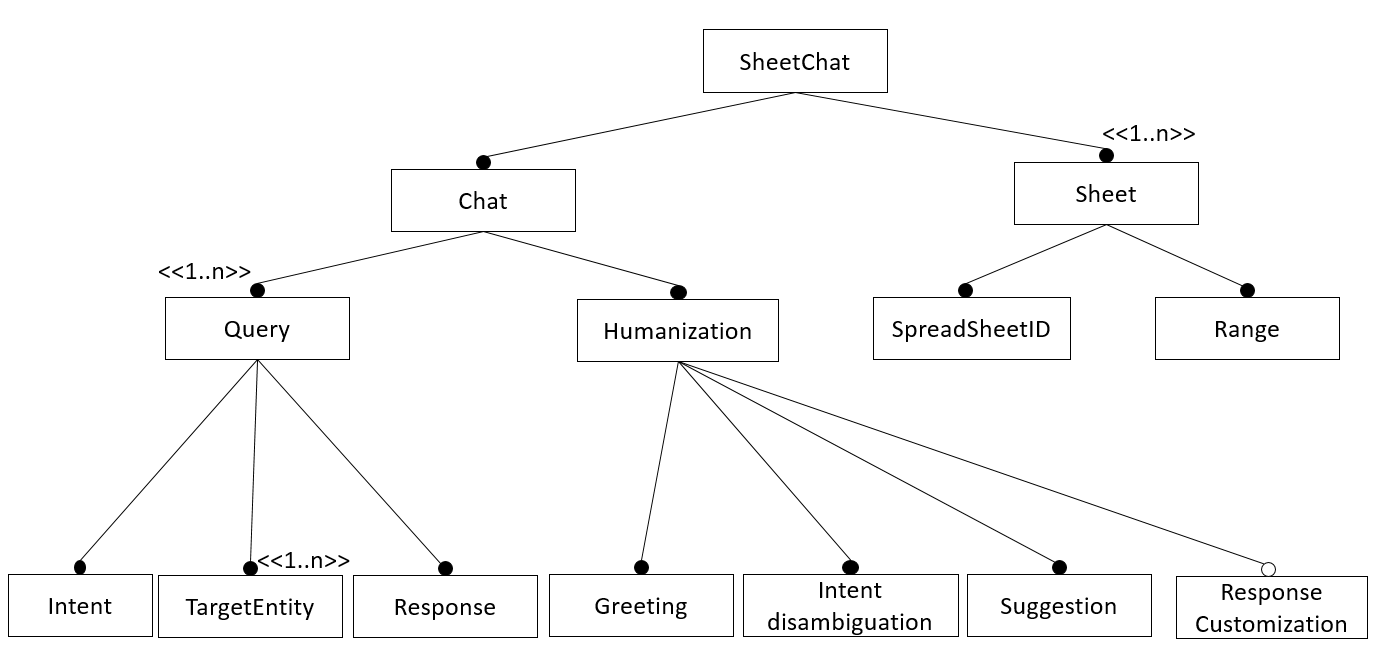
\includegraphics[width=0.8\textwidth]{./figs/FeatureModel.png}
	\caption{Modelo de características de SheetChat.} \label{fig:featureModel}
\end{figure}


En el Apartado \ref{sec:Sheet} se hablará sobre cómo se manejan las hojas de cálculo para su posterior consulta mediante un chatbot. En el Apartado \ref{sec:Chat} se describirá cómo se define un chatbot, el tipo de consultas y el procedimiento para hacerlas. Asimismo se mostrará el cómo se realiza la humanización de un chatbot, que permite mejorar la experiencia de usuario a la hora de conversar.

\section{Sheet}
\label{sec:Sheet}

Las hojas de cálculo son unas herramientas muy potentes que permiten además de generar gráficas o trabajar con complejas funciones matemáticas, el almacenar datos en forma matricial (filas y columnas). Las hojas de cálculo están orientadas al análisis de datos y las bases de datos al almacenamiento de las mismas \cite{Philips2014}, sin embargo, ambas almacenan datos basados en columnas y filas (o tuplas).

En el enfoque de nuestro trabajo, cada hoja de cálculo representa un conjunto de datos en forma de tabla. Al igual que sucede con los ficheros CSV, la primera fila es la cabecera de la tabla, donde se especifica cual es el nombre de cada columna. Las posteriores filas se traducen en tuplas que serán los datos a consultar.

A la hora de definir un chatbot se pueden definir más de un origen de datos. En la tecnología utilizada hay que mencionar que se definen hojas de cálculo en Google SpreadSheet\footnote{Sitio web de Google SpreadSheets: \url{https://www.google.com/sheets/about/}}. La principal ventaja que ofrece esta tecnología es que los datos residen en la nube, lo que permite ser accedidos desde cualquier plataforma y en cualquier momento y siempre se dispondrá de la versión más actualizada de los datos a consultar.

%TODO Explicar los dos campos para identificar el spreadsheet

Los datos que el usuario requiera consultar no serán datos en bruto, si no que el DSL desarrollado permitirá consultas con cierto nivel de riqueza. Para ello se ofrecen funciones matemáticas a la hora de mostrar el resultado o funciones de filtrado. Estas consultas se definen en el sistema de conversación de SheetChat en el Apartado \ref{sec:Consultas}.

\section{Chat}
\label{sec:Chat}

Tras definir el origen de los datos con el que trabajará el chatbot, se ha de definir la interfaz de consultas que tendrá el usuario al realizar las consultas a su hoja de cálculo. Antes de hablar del acceso a los datos, es importante destacar 

%TODO Intents y entities

\subsection{Consultas}
\label{sec:Consultas}

%TODO SQL engine

%TODO relación input-output column

%TODO entities en las que buscar

%TODO funcionalidades de output columns


\subsection{Humanizacion}
\label{sec:Humanization}

%TODO Greeting

%TODO Mensajes customizados

%TODO Mensajes de resultado no encontrado

%TODO Suggestions



\chapter{Construcción de bots mediante el DSL de SheetChat}

El diagrama de características estudiado previamente se ha de resolver en la definición de un chatbot. En este apartado se estudiará el DSL definido para la creación de un SheetChat. Para ello se tienen que tener en cuenta todas las características previamente mencionadas, la definición del origen de datos, la creación de una conversación que nos proporcione una petición de datos de entrada y su salida asociada; y no menos importante, recursos que nos permitan humanizar el bot para ofrecer una experiencia de usuario agradable.

Para ello en este trabajo se han elaborado tres ejemplos. El primero de ellos es dado las notas de dos asignaturas impartidas por un profesor de primaria, el poder preguntar por las notas de los alumnos que tiene. El segundo de los ejemplos permite dado un calendario de sesiones de un congreso científico, en este caso extraido del WISE de 2015\footnote{Calendario con las diferentes sesiones del congreso WISE: \url{http://www4.cis.fiu.edu/wise2015/@schema.html}}, poder obtener información sobre qué sesiones hay en los diferentes slots (u horarios). Por último, el tercer ejemplo permite, dada una hoja de cálculo autogenerada de una búsqueda de restaurantes de Miami en el sitio web Tripadvisor, obtener restaurantes por tipo de comida.

Cabe destacar que este DSL tiene múltiples objetivos:
\begin{itemize}
	\item El DSL debe ser fácilmente comprensible. Debe utilizar un lenguaje sencillo para la sintaxis concreta. En este caso se ha decidido implementarlo en JSON.
	\item El DSL debe de ser generable mediante una herramienta. La idea es que en un futuro este DSL sirva como base para una herramienta gráfica más sencilla de utilizar que ir escribiéndola de manera manual. Esto es debido al público objetivo, que son gente que desarrollan y utilizan hojas de cálculo en un dispositivo móvil; que carecerán de conocimiento de desarrollo de aplicaciones.
	\item El DSL debe permitir construir consultas complejas sin necesidad de hacer complejo el propio DSL.
	\item El DSL ha de abstraer de la implementación interna del bot y de las hojas de cálculo.
\end{itemize}

Partiendo de estas premisas, en la Figura \ref{fig:metamodel} se puede observar cuál es la sintaxis abstracta del DSL. Se define un SheetChat como una composición de un conjunto de Sheets y un Chat.

\begin{figure}[htb]
	\centering
	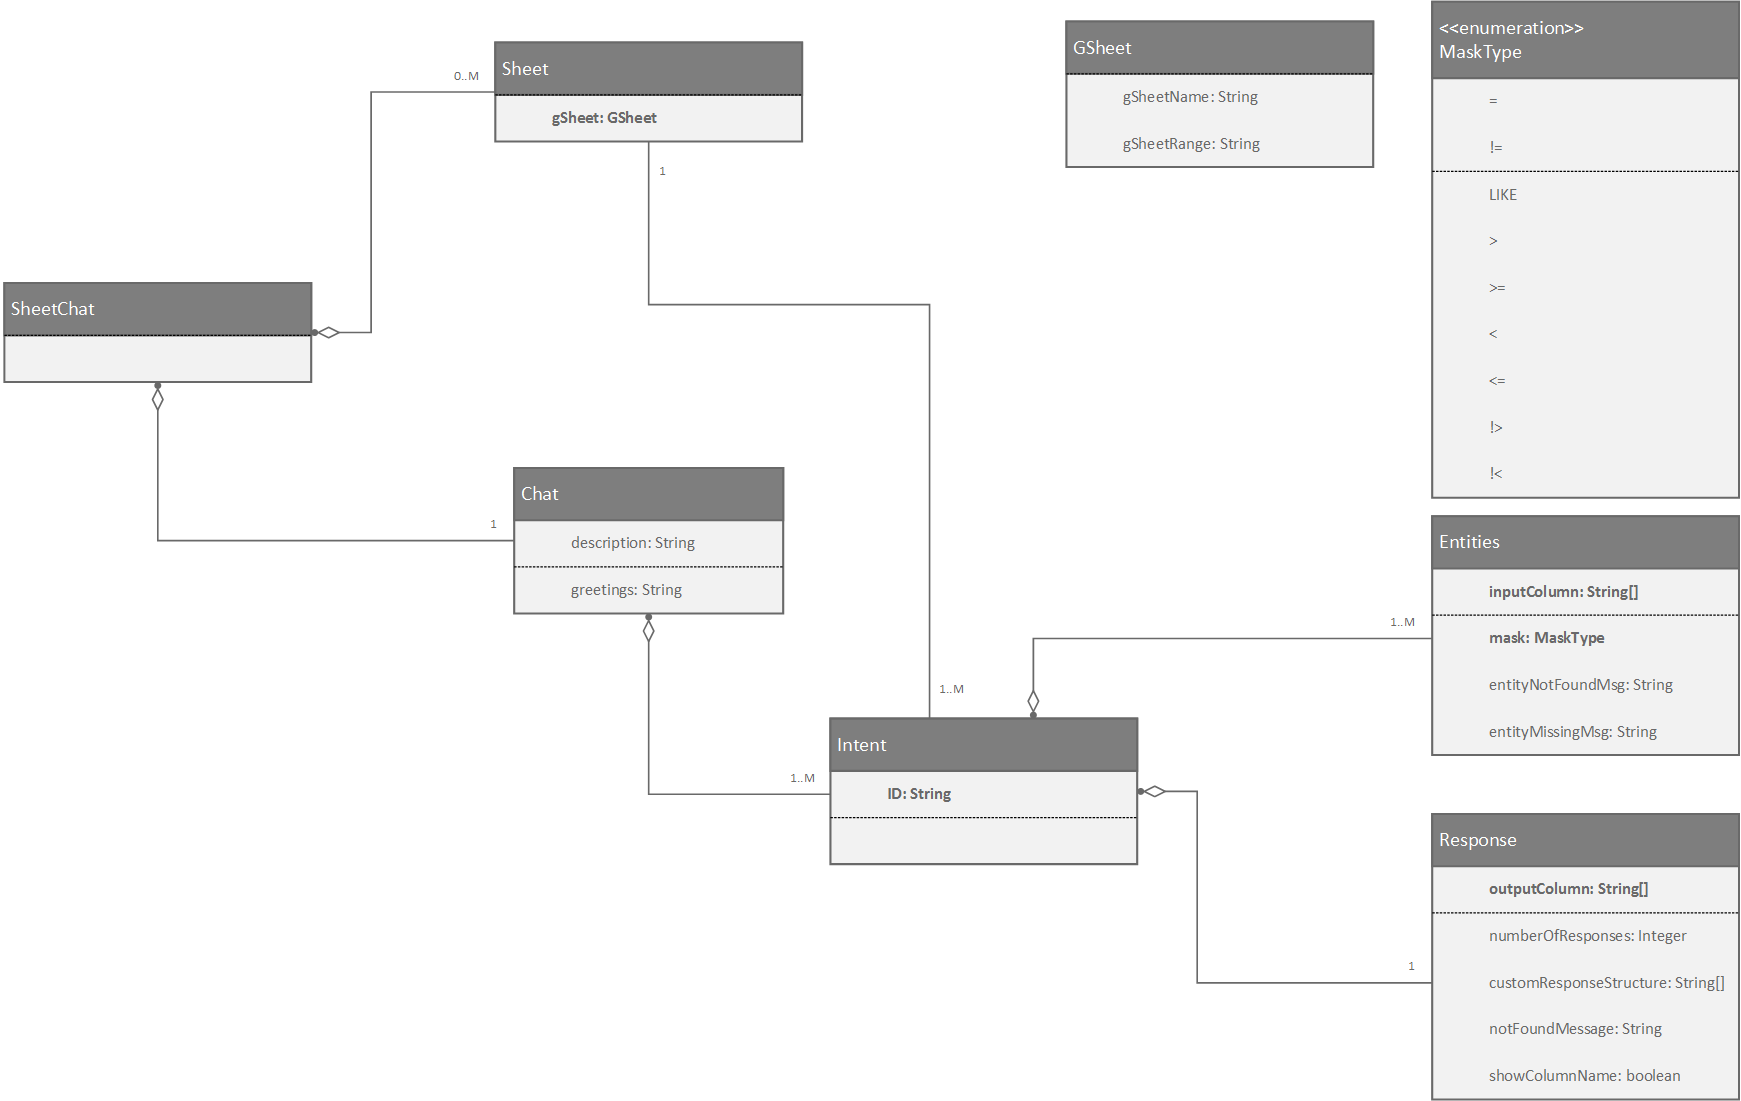
\includegraphics[width=0.8\textwidth]{./figs/Metamodel.png}
	\caption{Sintaxis abstracta del DSL para definir un SheetChat.} \label{fig:metamodel}
\end{figure}


Cada Sheet está representada por el nombre de la hoja de cálculo en Google SpreadSheets y el rango de las celdas que conforman la "tabla" sobre la que se consultará.

Cada Chat contendrá múltiples Intents. Cada uno de esos Intents tendrán un identificador único que estará relacionado con tipo de consulta que se le hará al Chatbot. Cabe destacar que los mensajes de Intents se infieren tras un entrenamiento a la herramienta Wit.ai mencionada en el Apartado \ref{sec:Humanization}. Por cada Intent habrá una respuesta que el chatbot proporcionará con el resultado extraído de la hoja de cálculo y un número de entidades que funcionarán a modo de filtrado para obtener ese resultado.

\section{Ejemplo 1: Notas de asignaturas impartidas por un profesor}

El uso de hojas de cálculo para almacenar las notas de los alumnos por parte del profesorado es una práctica habitual. Quizá un profesor no tenga una necesidad imperiosa de utilizar esta hoja de cálculo de manera móvil, pero es un ejemplo sencillo y claro para mostrar las características del DSL desarrollado.

La idea es que un profesor tenga 


\section{Ejemplo 2: Calendario de sesiones en un congreso científico}

Los congresos científicos aúnan conocimiento de distinta índole. Habitualmente estos eventos disponen de un calendario complejo, dónde hay trabajos más o menos interesantes o relevantes con la rama de especialización que tiene el asistente. Es por ello que acudir a las sesiones más afines a tu trabajo es importante. Es interesante disponer de información in situ de cuales son las próximas charlas que habrá, dónde o quién las presenta. Sin embargo, los sitios webs rara vez están preparados para su navegación por el móvil o se pierde mucho tiempo en encontrar los eventos a los que se desea acudir. Es una información relevante y que se desea conocer en el momento. 

En este ejemplo se trata de definir un Chatbot que permita consultar información relacionada con las diferentes sesiones de un congreso. Para ello el ejemplo se basa en extraer una tabla con el calendario del mismo y definir diferentes consultas sobre los datos. Para este ejemplo se han definido dos cuestiones habituales que suele tener un asistente a un congreso: 
\begin{itemize}
	\item \textbf{¿Cuáles son las charlas en un horario concreto, es decir, qué eventos hay en esa franja horaria?} De los eventos que existan en esa franja horaria, el asistente al congreso podría decantarse por la que más interesante le resulte.
	\item \textbf{¿Qué eventos hay relacionados con un tema (o topic) en particular?} De esta manera el usuario sabrá con una simple pregunta qué eventos le pueden resultar interesantes.
\end{itemize}



\section{Ejemplo 3: Búsqueda de restaurantes de Tripadvisor}



\chapter{Trabajo Futuro y Conclusiones}
\label{cha:FutureWorkAndConclusions}

En este capítulo se divide en dos apartados. En el Apartado \ref{sec:FutureWork} se hablará del trabajo futuro y de las mejoras que se puedan aplicar a este trabajo. En el Apartado \ref{sec:Conclusions} se extraerán unas conclusiones obtenidas durante el desarrollo del trabajo.

\section{Trabajo futuro}
\label{sec:FutureWork}

El trabajo presentado en este proyecto sirve como prueba conceptual para demostrar que la solución al problema detectado puede ser factible. Está claro que un componente que demostrará, si además de ser factible, es útil es la evaluación de la propia herramienta con usuarios de hoja de cálculo. Es por ello que resulta difícil de vaticinar cuales son los siguientes pasos a dar en el desarrollo de esta idea, ya que irán claramente asociada a esa evaluación y feedback que puedan proporcionar los usuarios.

Sin embargo, a lo largo del desarrollo se han detectado algunos aspectos de mejora en lo que a la herramienta se refiere. En concreto se han dividido en los siguientes aspectos: enriquecimiento del diseño del DSL, usabilidad de los chatbot generados, el ecosistema de plataformas utilizado para su desarrollo y la actualización de los datos de las hojas de cálculo.

\subsection{Diseño del DSL}

El DSL diseñado permite la creación de consultas abstrayendo al usuario del conocimiento de un lenguaje como es SQL. A pesar de que esto resulta positivo, se ha detectado que el actual diseño del DSL no permite realizar consultas que puede que sean bastantes habituales, especialmente sobre datos tabulares extraídos de sitios web de manera automática.

De igual manera, el lenguaje de tipado JSON, a pesar de que sea legible por el humano y fácilmente generable, no es un lenguaje con el que el usuario se sienta excesivamente cómodo. Esto es debido a que el usuario final de esta herramienta es posible que no conozca JSON. A pesar de que no hay una evaluación de por medio, es posible que utilizar hojas de cálculo también para definir los chatbots sea más intuitivo para los usuarios.

Como se ha comentado a lo largo del trabajo, la idea es que una herramienta, posiblemente gráfica, sea capaz de ayudar (o sustituir) en la elaboración de este esquema para definir las propiedades necesarias para la creación de un Sheetchat. En esta herramienta será fundamental ver cuánto se requiere para la realización de un chatbot que cubra las necesidades de los usuarios.

\subsection{Usabilidad de los Chatbot generados}

El sistema de sugerencias desarrollado es bastante espartano, ya que se utiliza una función de aleatorización para ir mostrando diferentes sugerencias cada vez que el usuario introduzca entidades que no existen. Sin embargo puede ser que el usuario esté cometiendo un error tipográfico y que el bot le esté indicando constantemente que esa entidad no existe. En este caso, la experiencia de usuario mejoraría considerablemente.

A pesar de que se ha trabajado en aspectos de humanización, hay que ver si son realmente útiles o suficientes. También sería conveniente ver si hay más patrones de diseño de chatbots de manera que se pueda equiparar los chatbots que hay en el mercado con los que se generan con esta herramienta. Aplicando un patrón de diseño se obtienen chatbots con funcionalidades similares, lo que simplificaría el proceso de aprendizaje para usar el chatbot.

\subsection{Ecosistema de plataformas}

Sería conveniente realizar un estudio más en profundidad de las plataformas y librerías para desarrollo y despliegue de agentes conversacionales.

Para este trabajo se ha utilizado Botkit, que es una librería muy sencilla y muy potente junto con el middleware de Wit.ai. Sin embargo, su desarrollo no es demasiado continuado y solo ofrece soporte para tres plataformas como son Slack, Facebook Messenger y Twilio. 

Entre las alternativas, Microsoft Bot Framework está cogiendo mucha fuerza debido a que es capaz de generar bots para muchas más plataformas. Sería interesante ver qué plataformas son las más usadas. La tendencia actual es que Facebook Messenger y Slack son de las más utilizadas \footnote{Encuesta a la comunidad de desarrolladores de chatbots: \url{http://venturebeat.com/2016/09/14/early-results-of-bot-community-survey-show-messenger-and-slack-as-the-developers-top-platforms/}}.

\subsection{Hojas de cálculo}

El principal handicap de las hojas de cálculo que tienen datos extraídos de sitios web mediante herramientas automatizadas es que debe el usuario actualizarlas de manera manual cada cierto tiempo.

En la actualidad para solventar ese problema se ha detectado la existencia de dos herramientas que habría que ver si pueden ser interesantes implantarlas en el ecosistema de SheetChat.

Las propias hojas de cálculo de google tienen una funcionalidad que es exportar una tabla html de un sitio web \footnote{Tutorial de uso de la función de Google Sheets importhtml: \url{https://mashe.hawksey.info/2012/09/reshaping-importhtml-data-in-google-spreadsheet-using-query-and-transpose-formula/}} y que se actualizará de manera automática. A pesar de que en la mayoría de los casos no trabaje bien, ya que depende de la correcta estructuración de la tabla html, puede servir para datos que están bien estructurados.

Además de los sitios web html como fuente de información, los servicios web RESTful o SOAP también contienen una cantidad de información fácilmente accesible. Existe una solución que permite extraer hojas de cálculo dado un endpoint de un servicio RESTful \cite{Chang2014}.

\section{Conclusiones}
\label{sec:Conclusions}

El desarrollo de este trabajo ha permitido ofrecer una respuesta a la problemática de cómo acceder a datos de una hoja de cálculo en un entorno móvil.

Lo novedoso de la solución es que utiliza el lenguaje natural como interfaz para realizar consultas a una hoja de cálculo \cite{Flood2010}. La generación de consultas SQL a partir de las definiciones de Intents y Entidades proporciona una abstracción sobre el propio lenguaje SQL. Para gente que no tenga conocimientos de SQL poder consultar en bases de datos utilizando el lenguaje natural es muy ventajoso. Sin embargo, a la vez que la generación de consultas SQL a partir de Intents y Entidades tiene sus ventajas, la limitación que tiene también queda patente.

Los aspectos de humanización en un chatbot son fundamentales, incluso siendo para autoconsumo en el que el usuario/desarrollador conozca todos los aspectos del chatbot. Estos aspectos de humanización presentan una interfaz más cercana al usuario y mejoran la experiencia de usuario reduciendo costes temporales.

Aplicando patrones de diseño como el de obligar a definir un mensaje de bienvenida se resuelven muchos problemas. Estos problemas, aunque parezca increible, hay muchos bots de terceros en la web que tienen esta carencia.Esto provoca que un usuario descarte la posibilidad de usar este chatbot porque no puede sabe ni tan siquiera qué hace el bot.
























% line in order to check if utf-8 is properly configured: áéíóúñ


%%%%%%%%%%%%%%%%%%%%%%%%%
%%% End content files %%%
%%%%%%%%%%%%%%%%%%%%%%%%%

\noappendicestocpagenum
\appendixpage
\addappheadtotoc
\appendix
% Adjustments headers
\pagestyle{fancy}
\fancyhead[LO]{\leftmark}
\ifdefined\euskaraz
	\fancyhead[RE]{\emph{\thechapter eranskina}}
\else
	\fancyhead[RE]{\emph{Anexo \thechapter}}
\fi
\renewcommand{\headrulewidth}{0.5pt}

% \chapter{Import.io: Extracción de datos tabulares a partir de la web}
\label{anx:importio}

Import.io es una herramienta que permite extraer datos de un sitio web de manera sencilla y convertirlos a datos en forma de tabla, concretamente a ficheros CSV. A estos artefactos de extracción de datos se les denomina extractores. Un extractor es representado por un número de URLs o direcciones web que tendrá como origen de datos y el método de extracción de datos, es decir, qué elementos de un sitio web corresponden a qué columna de la tabla que se va a extraer.

Import.io es capaz de inferir todas las URLs que pueden ser relevantes proporcionándole algunos ejemplos si todas estas comparten alguna característica o estructura similar. En la Figura \ref{fig:ImportioURLs} se puede observar cómo se han generado URLs con las diferentes páginas de búsqueda de restaurantes en Miami en el sitio web Tripadvisor\footnote{Búsqueda de restaurantes en Miami en Tripadvisor: \url{https://www.tripadvisor.co.uk/RestaurantSearch-g34438-oa30-Miami_Florida.html}}

\begin{figure}[htb]
	\centering
	\includegraphics[width=0.8\textwidth]{./figs/ImportioURLs.png}
	\caption{Generador de URLs en las que extraer datos para import.io.}
	\label{fig:ImportioURLs}
\end{figure}

Import.io mediante el uso de heurísticos define qué datos siguen un patrón concreto dentro de un sitio web y los marca como candidatos a formar parte de la tabla resultante. Sin embargo, una característica muy interesante es poder definir las columnas a qué elementos del sitio web hacen referencia. En la Figura \ref{fig:ImportioEdit} está en el panel superior marcada la columna de \emph{Image} y te marca el elemento HTML con el que hacer el matching.

\begin{figure}[htb]
	\centering
	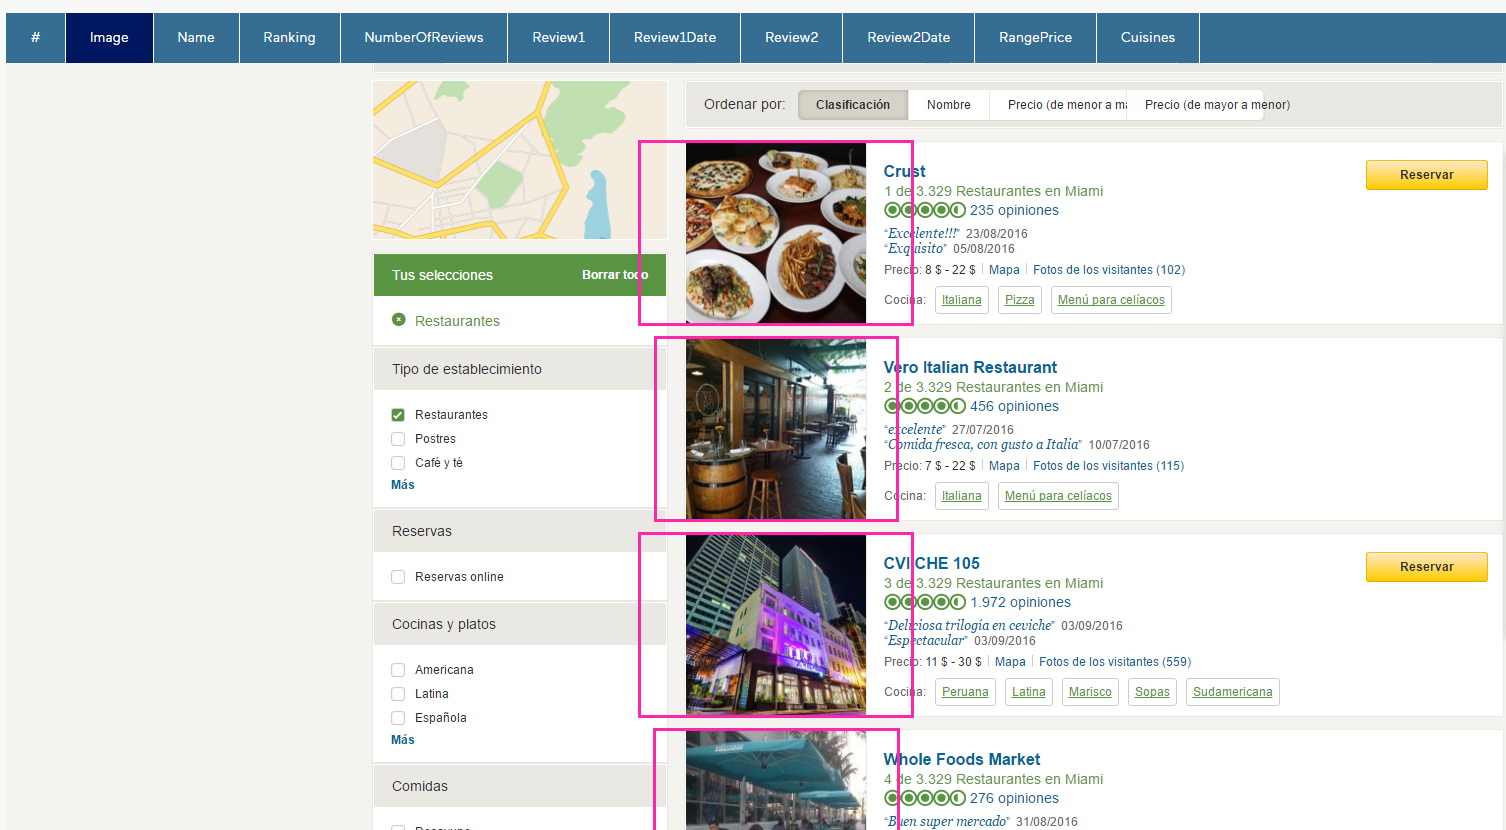
\includegraphics[width=0.8\textwidth]{./figs/ImportioEdit.png}
	\caption{Pantalla de edición de los elementos HTML a extraer en la tabla generada por import.io.}
	\label{fig:ImportioEdit}
\end{figure}

Como última característica, cabe destacar que import.io, en su versión de pago, permite la actualización automática de los cambios que se produjesen en la hoja de cálculo resultante. Es decir, en caso de que el sitio web cambiase, algo muy frecuente en sitios web de esta índole, import.io se encargaría de escanear y extraer la tabla con el formato que se haya preestablecido.

Al igual que existe import.io, existen otras herramientas para la extracción de datos en forma tabular:
\begin{itemize}
	\item \textbf{importhtml de Google Spreadsheets}\footnote{Extracción de datos con importhtml de Google SpreadSheets: \url{https://mashe.hawksey.info/2012/09/reshaping-importhtml-data-in-google-spreadsheet-using-query-and-transpose-formula/}}, menos potentes, pero mucho más sencilla de utilizar y con contenido actualizable.
	\item \textbf{Gneiss Spreadsheet} permite definir consultas y extraer datos en forma de tabla de un servicio web RESTful API \cite{Chang2014} con la funcionalidad de auto-actualización de los datos.
\end{itemize}

\chapter{Wit.ai: Procesamiento del lenguaje natural orientado a bots conversacionales}
\label{anx:witai}

Wit.ai se define como una herramienta de procesamiento del lenguaje, ya sea para texto como para voz. El objetivo de esta herramienta es funcionar de nexo entre el lenguaje que comprenden los humanos y las funcionalidades que dispone un sistema software, como lo puede ser un chatbot. Trabaja con diferentes lenguajes como el inglés o el castellano (en fase de desarrollo actualmente, aunque funciona relativamente bien). La principal virtud es que con poco trabajo Wit.ai empieza a funcionar como es esperado. Wit.ai funciona a base de entrenamiento, es decir, el desarrollador de la aplicación debe de ir introduciendo frases que el usuario utilizaría para hacer peticiones al sistema. A medida de que disponga de más frases más preciso será encontrando las intenciones (Intents) o entidades que los usuarios hayan introducido.

Respecto al trabajo referente a SheetChat, se ha delegado la tarea de desambiguación de Intents y reconocimiento de entidades a Wit.ai. Wit.ai permite tanto introducir frases de manera manual o esperar a recibir frases de los usuarios e ir corrigiendo desambiguaciones en las que se haya podido equivocar Wit.ai para mejorar su sistema de reconocimiento. En la Figura \ref{fig:WitaiInbox} se pueden observar dos mensajes introducidos por alguno de sus usuarios. El sistema ha reconocido tanto la entidad alumno como el Intent al que se refería el usuario. Sin embargo en la Figura \ref{fig:WitaiFallo} Wit.ai ha sido incapaz de obtener toda la información necesaria para resolver la pregunta del usuario. En la imagen superior ha reconocido erroneamente el Intent y no ha visto la entidad alumno (lo que indica que requiere más entrenamiento con frases de ese tipo). En la imagen inferior si ha sido capaz de reconocer adecuadamente el Intent, pero no ha podido obtener la entidad alumno, por lo que tendrá que preguntar por ella para dar respuesta al Intent.

\begin{figure}[htb]
	\centering
	\includegraphics[width=0.8\textwidth]{./figs/WitaiInbox.png}
	\caption{Wit.ai infiriendo de dos frases cuales son los Intents correspondientes para cada uno de ellos y cuál es la entidad Alumno.}
	\label{fig:WitaiInbox}
\end{figure}

\begin{figure}[htb]
	\centering
	\includegraphics[width=0.8\textwidth]{./figs/WitaiFallo.png}
	\caption{En la imagen de arriba Witai infiere erroneamente el Intent y no reconoce la entidad. En la inferior el usuario no ha proporcionado ninguna entidad, por lo que el chat tendrá que preguntar por ella.}
	\label{fig:WitaiFallo}
\end{figure}

Como se ha mencionado previamente, Wit.ai funciona en base a una confianza en las detecciones que ha hecho. En SheetChat se exige que el grado de confianza ha de ser mayor que 0.5 sobre 1 para que una inferencia se de por válida. En la Figura \ref{fig:WitaiConfianza} se puede observar como el grado de confianza de que \emph{María} es un alumno es de 0.99 y que el Intent es \emph{fisicaPonderadaPorEjercicio} únicamente de 0.71. Si se le ha entrenado adecuadamente, es muy probable que María sea un alumno y, con una confianza menor, que lo que se quiere es obtener la media ponderada de los ejercicios de física.

\begin{figure}[htb]
	\centering
	\includegraphics[width=0.8\textwidth]{./figs/WitaiConfianza.png}
	\caption{Respuesta del servicio de wit.ai cuando se le proporciona una frase. Remarcado en morado está el grado de confianza referente a la entidad alumno que ha detectado, de azul la del Intent.}
	\label{fig:WitaiConfianza}
\end{figure}




























% line in order to check if utf-8 is properly configured: áéíóúñ



\backmatter

\bibliography{gap-pfg}

\chapter{Agradecimientos}

En primer lugar, me gustaría agradecer a mi director de proyecto Óscar Díaz por confiar en mi para la realización de este TFM. Ha sabido guiarme correctamente a lo largo de la elaboración del trabajo, atendiendo a las consultas con un trato humano excepcional.

Asimismo, me gustaría agradecer a mis compañeros de trabajo dentro del grupo Onekin. Estos no solo me han brindado con su ayuda cuando la he necesitado, si no que también me han abierto las puertas de su grupo de par en par haciéndome sentir uno más del equipo.

De igual manera, quiero agradecer a mis compañeros de clase, de los que en poco tiempo he adquirido mucho conocimiento que me será útil para desarrollarme tanto profesionalmente como en el ámbito personal.

Por último, agradecer a mi familia, amigos, a Ainhoa y a mi entorno más cercano que una vez más han confiado en mi y me han respaldado en todo lo que he necesitado.

% In case we are using a glossary
% \glstoctrue
% \glsaddall
% \printglossaries

\end{document}
% line in order to check if utf-8 is properly configured: áéíóúñ
